
% v2-acmsmall-sample.tex, dated March 6 2012
% This is a sample file for ACM small trim journals
%
% Compilation using 'acmsmall.cls' - version 1.3 (March 2012), Aptara Inc.
% (c) 2010 Association for Computing Machinery (ACM)
%
% Questions/Suggestions/Feedback should be addressed to => "acmtexsupport@aptaracorp.com".
% Users can also go through the FAQs available on the journal's submission webpage.
%
% Steps to compile: latex, bibtex, latex latex
%
% For tracking purposes => this is v1.3 - March 2012
\documentclass[prodmode,acmtecs]{acmsmall} % Aptara syntax
\usepackage[spanish,polish]{babel}
\usepackage[T1]{fontenc}
\usepackage{fancyvrb}
\usepackage{graphicx,hyperref}
\newcommand\cutout[1]{}


\usepackage[table]{xcolor}
\usepackage[utf8]{inputenc}
\usepackage[parfill]{parskip}
\usepackage{tabulary}
\PassOptionsToPackage{hyphens}{url}
\usepackage{hyperref}    
\usepackage[capitalize]{cleveref}


% Metadata Information
% !!! TODO: SET THESE VALUES !!!
\acmVolume{0}
\acmNumber{0}
\acmArticle{CFP}
\acmYear{0}
\acmMonth{0}

\newcounter{colstart}
\setcounter{page}{4}

\RecustomVerbatimCommand{\VerbatimInput}{VerbatimInput}%
{
%fontsize=\footnotesize,
fontfamily=\rmdefault
}


\newcommand{\UnderscoreCommands}{%\do\verbatiminput%
\do\citeNP \do\citeA \do\citeANP \do\citeN \do\shortcite%
\do\shortciteNP \do\shortciteA \do\shortciteANP \do\shortciteN%
\do\citeyear \do\citeyearNP%
}

\usepackage[strings]{underscore}



% Document starts
\begin{document}


\setcounter{colstart}{\thepage}

\acmArticle{CFP}
\title{{\huge\sc SIGLOG Monthly 234}

 February 2023}
\author{DAVID PURSER\affil{University of Liverpool, UK}
\vspace*{-2.6cm}\begin{flushright}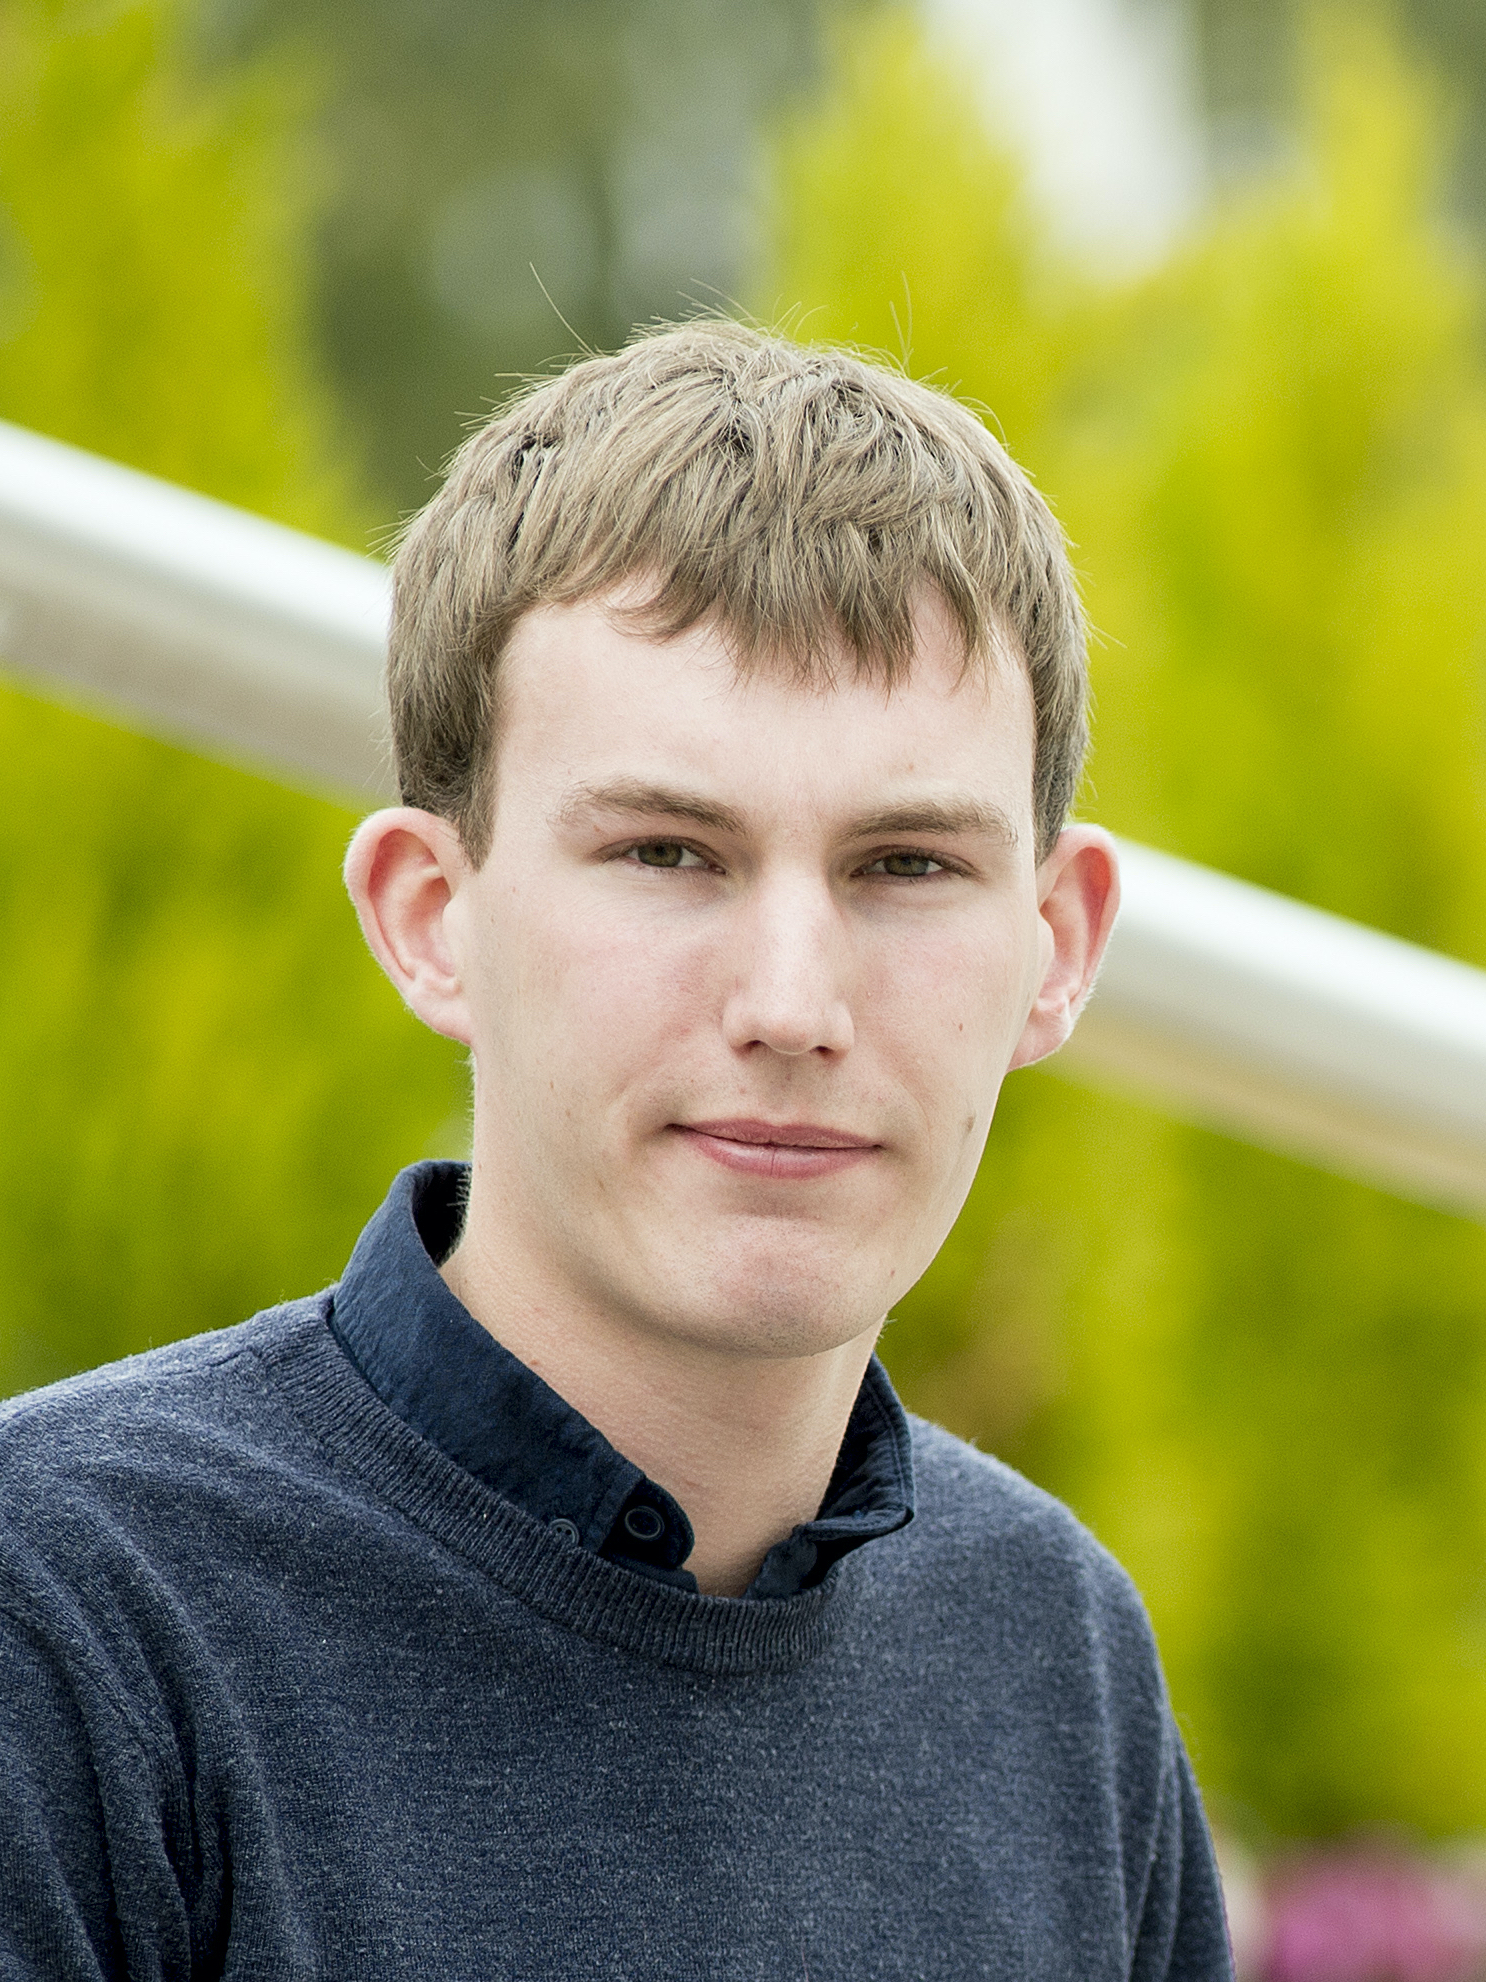
\includegraphics[width=30mm]{dp}\end{flushright}
}

\begin{abstract}
February 2023 edition of SIGLOG Monthly, featuring deadlines, calls and community announcements.
\end{abstract}


\maketitlee

\href{https://lics.siglog.org/newsletters/}{Past Issues}
 - 
\href{https://lics.siglog.org/newsletters/inst.html}{How to submit an announcement}
\section{Table of Content}\begin{itemize}\item DEADLINES (\cref{deadlines}) 
 
\item CALLS 
 
\begin{itemize}\item IJCAI 2023 (CALL FOR WORKSHOPS) (\cref{IJCAI2023})
\item DEON 2023 (CALL FOR PAPERS) (\cref{DEON2023})
\item ICDT 2024 (CALL FOR PAPERS) (\cref{ICDT2024})
\item MARKTOBERDORF 2023 (CALL FOR PARTICIPATION) (\cref{MARKTOBERDORF2023})
\item CLAR 2023 (CALL FOR PAPERS) (\cref{CLAR2023})
\item GCM 2023 (CALL FOR PAPERS) (\cref{GCM2023})
\end{itemize} 
\item JOB ANNOUNCEMENTS 
 
\begin{itemize}\item Assistant Professor in Theoretical Computer Science in Amsterdam (\cref{AssistantProfessorinTheoreticalComputerScienceinAmsterdam})
\item Faculty Positions at the University of Quebec in Montreal (\cref{FacultyPositionsattheUniversityofQuebecinMontreal})
\end{itemize} 
\end{itemize}\section{Deadlines}\label{deadlines}\rowcolors{1}{white}{gray!25}\begin{tabulary}{\linewidth}{LL}Alonzo Church Award 2023:  & Feb 01, 2023 (Deadline for nominations) \\
CONFEST 2023:  & Feb 02, 2023 (Submission deadline) \\
CAV 2023:  & Feb 03, 2023 (Paper), Apr 25, 2023 (Artifact), Feb 20, 2023 (CAV AWARD Nomination deadline) \\
IJCAI 2023:  & Feb 03, 2023 (Proposal  deadline) \\
FSCD 2023:  & Feb 04, 2023 (Abstract, Extended), Feb 09, 2023 (Paper, Extended) \\
CiE 2023:  & Feb 08, 2023 (Abstract), Feb 15, 2023 (Article) \\
ICALP 2023:  & Feb 11, 2023 at 11am CET (Paper) \\
POSTDOC POSITION in WARSAW:  & Feb 15, 2023 (Applications) \\
Salomaa Prize:  & Feb 28, 2023 (Deadline for nominations) \\
ICGT 2023:  & Feb 28, 2023 (Abstract), Mar 07, 2023 (Paper) \\
LOGIC COLLOQUIUM 2023:  & Mar 01, 2023 (Abstract), Mar 01, 2023 (Student Travel Grants deadline) \\
DEON 2023:  & Mar 01, 2023 (Abstract), Mar 31, 2023 (Paper) \\
Assistant Professor in Theoretical Computer Science in Amsterdam:  & Mar 14, 2023 (Deadline for application) \\
ICDT 2024:  & Mar 20, 2023 (Cycle 1 Abstract), Mar 27, 2023 (Cycle 1 Full Submission due), Sep 13, 2023 (Cycle 2 Abstract), Sep 20, 2023 (Cycle 2 Full) \\
Faculty Positions at the University of Quebec in Montreal:  & Mar 31, 2023 (Application deadline) \\
CLAR 2023:  & Apr 10, 2023 (Submission deadline) \\
MARKTOBERDORF 2023:  & Apr 15, 2023 (Registration deadline) \\
FORMATS 2023:  & Apr 21, 2023 (Abstract), Apr 28, 2023 (Paper) \\
ICLP 2023:  & Apr 28, 2023 (non-regular paper) \\
GCM 2023:  & May 07, 2023 (Abstract), May 14, 2023 (Paper) \\
\end{tabulary}
\section{IJCAI 2023: 32nd International Joint Conference on Artificial Intelligence}\label{IJCAI2023}  August 19-25, 2023\\ 
  Cape Town, South Africa\\ 
CALL FOR WORKSHOPS 

\begin{itemize}\item  The 32nd International Joint Conference on Artificial Intelligence (IJCAI 2023) is inviting proposals for workshops to be held August 19-21, 2023, in Cape Town, South Africa, immediately before the main conference. 
 
  All the details can be found here: \href{https://ijcai-23.org/call-for-workshop-proposals/}{https://ijcai-23.org/call-for-workshop-proposals/} 
 
  The important dates are: (anywhere on earth) 
 
\rowcolors{1}{white}{gray!25}\begin{tabulary}{\linewidth}{LL}Proposal submission deadline:  & Feb 03, 2023 \\
Acceptance notification:  & Mar 06, 2023 \\
IJCAI 2023 workshops:  & Aug 19-21, 2023 \\
\end{tabulary}
 
  We look forward to receiving your proposals! Should you have any question about the workshops, feel free to reach us at the email workshops@ijcai-23.org. 
 
\end{itemize}\section{DEON 2023: 16th INTERNATIONAL CONFERENCE ON DEONTIC LOGIC AND NORMATIVE SYSTEMS}\label{DEON2023}  July 5-7, 2023, Trois-Rivières, Canada\\ 
  \href{http://www.uqtr.ca/DEON2023}{http://www.uqtr.ca/DEON2023}\\ 
CALL FOR PAPERS 

\begin{itemize}\item  DEON 2023 will focus on the theme Theoretical and technical limitations of automated behavior. 
 
\item  IMPORTANT DATES 
 
\rowcolors{1}{white}{gray!25}\begin{tabulary}{\linewidth}{LL}Abstract submission:  & Mar 01, 2023 \\
Paper submission:  & Mar 31, 2023 \\
\end{tabulary}
 
\item  INVITED SPEAKERS 
 
\begin{itemize}\item Lou Goble (Willamette University), Pedro Cabalar (Corunna University),
\item  Huimin Dong (Sun Yat-Sen University), other speakers TBA.
\end{itemize} 
\item  Detailed information can be found on the webpage. 
 
\end{itemize}\section{ICDT 2024: 27th INTERNATIONAL CONFERENCE ON DATABASE THEORY}\label{ICDT2024}  Paestum, Italy, March 25-28, 2024\\ 
  For more info check \href{https://dastlab.github.io/edbticdt2024/}{https://dastlab.github.io/edbticdt2024/}\\ 
CALL FOR PAPERS 

\begin{itemize}\item  ICDT is a series of international scientific conferences on research of data management theory (\href{https://databasetheory.org/icdt-pages}{https://databasetheory.org/icdt-pages}). The 27th edition of ICDT, in 2024, will take place in Paestum, Italy. 
 
\item  TOPICS OF INTEREST 
 
    We welcome research papers onevery topic related to the principles and theory of data management, provided that there is a clear connection to foundational aspects. 
 
  This includes, for example, articles on ``classical'' data management topics such as: 
 
\begin{itemize}\item  The design and study of data models and query languages
\item  The development and analysis of algorithms for data management
\item  The theoretical investigation of various aspects underlying data management systems (indexes, concurrency, distributed computation, privacy and security, ...)
\end{itemize} 
  but also includes papers exploring existing or identifying new connections between data management and other areas, such as the areas of: 
 
\begin{itemize}\item  knowledge representation, semantic web
\item  information retrieval and data mining
\item  machine learning/AI
\item  distributed computing
\item  theoretical computer science.
\end{itemize} 
\item  IMPORTANT DATES  
 
  ICDT will have two submission cycles for 2024, with deadlines as follows: 
 
\rowcolors{1}{white}{gray!25}\begin{tabulary}{\linewidth}{LL}Cycle 1 Abstract submission:  & Mar 20, 2023 \\
Cycle 1 Full Submission due:  & Mar 27, 2023 \\
Cycle 1 Notification:  & Jun 05, 2023 \\
Cycle 2 Abstract submission:  & Sep 13, 2023 \\
Cycle 2 Full submission:  & Sep 20, 2023 \\
Cycle 2 Notification:  & Nov 29, 2023 \\
\end{tabulary}
 
\item  Submission instructions can be found on the webpage 
 
\end{itemize}\section{MARKTOBERDORF 2023: MARKTOBERDORF SUMMER SCHOOL 2023 ON SAFETY AND SECURITY THROUGH FORMAL VERIFICATION}\label{MARKTOBERDORF2023}  August 2-11, 2023\\ 
  \href{https://events.model.in.tum.de/mod23}{https://events.model.in.tum.de/mod23}\\ 
CALL FOR PARTICIPATION 

\begin{itemize}\item  The ``Marktoberdorf Summer School'' is an 11-day event for young computer scientists and mathematicians, typically doctoral and post-doctoral researchers. It provides mini-courses on state-of-the-art topics in ``Safety and Security through Formal Verification'' and leaves ample room for interaction between participants and speakers. 
 
\item  REGISTRATION 
 
  Registration opens on February 2023. Register online at 
 
  \href{https://events.model.in.tum.de/mod23/participation.html}{https://events.model.in.tum.de/mod23/participation.html} 
 
Registration deadline: Apr 15, 2023 
 
\item  SPEAKERS AND COURSES: 
 
\begin{itemize}\item  PAROSH AZIZ ABDULLA: Algorithmic Verification of Infinite-State Systems
\item  JASMIN BLANCHETTE: Solvers and Provers
\item  BYRON COOK: Cloud Reasoning
\item  JAVIER ESPARZA: Interactive Proof Systems: From Theory to Practice
\item  JAN KRETINSKY: Learning-Aided Probabilistic Verification and Synthesis
\item  ANCA MUSCHOLL Distributed synthesis and control
\item  ALEKSANDAR NANEVSKI: Type and Proof Structures for Concurrent Programs
\item  CORINA PASAREANU: Symbolic Execution and Quantitative Reasoning: Applications to Software Safety and Security
\item  GRIGORE ROSU: Automated Synthesis of Temporal-Logic Specifications
\item  JAMES WORRELL: Orbit Problems for Dynamical Systems
\item  HONGSEOK YANG: Probabilistic Programming 
\end{itemize} 
\end{itemize}\section{CLAR 2023: The 5th International Conference on Logic and Argumentation}\label{CLAR2023}  September 10-12, 2023, Hangzhou (China)\\ 
  \href{https://www.zlaire.net/clar2023/}{https://www.zlaire.net/clar2023/}\\ 
CALL FOR PAPERS 

\begin{itemize}\item  CLAR 2023 
 
  The 5th International Conference on Logic and Argumentation (CLAR 2023) invites contributions from logic, artificial intelligence, philosophy, computer science, linguistics, law, and other areas studying logic and formal argumentation. CLAR 2023 will be held 10th-12th September 2023 at Zhejiang University in Hangzhou.  
 
  CLAR 2023 aims to highlight recent advances in logic and argumentation and foster interaction in these two areas between researchers within and outside China. 
 
   The interplay between logic and argumentation spans different disciplines and historical eras: from ancient philosophy (Socrates' dialectics, Aristotle's logic) to contemporary computer science (dialogues, multiagent systems). Research in logic and argumentation offers formal or semi-formal models that capture reasoning patterns and dialogue activities of diverse kinds. Their applications in artificial intelligence range from law and ethics to linguistics. CLAR 2023 will focus on a variety of topics and formalisms, including formal models of argumentation (abstract or structured), preference and support, but also dispute and dialogue systems for online argumentation or the processing of legal texts. 
 
  Established in 2016 as a workshop hosted by Zhejiang University, the CLAR series has been increasingly successful and become an international event and discussion forum in the two areas of logic and argumentation. Our aim for CLAR 2023 is to be a platform for the advancement of the existing discussions within each of the areas above, to span bridges between their different traditions, and finally to open argumentation to new applications and other areas in artificial intelligence, such as legal reasoning, explainable AI, ethical dilemmas, reasoning about uncertainty and knowledge representation, etc. Previous conferences can be accessed via: \href{http://www.xixilogic.org/events/clar}{http://www.xixilogic.org/events/clar}. 
 
  CLAR 2023 will be financially supported by a national key project called ``Research on Logics for New Generation Artificial Intelligence'' (2021-2025), granted by the National Social Science Foundation of China. Information about the project: \href{https://xixilogic.org/lngai/}{https://xixilogic.org/lngai/}. 
 
\item  IMPORTANT DATES 
 
\rowcolors{1}{white}{gray!25}\begin{tabulary}{\linewidth}{LL}Submission deadline:  & Apr 10, 2023 \\
Notification:  & Jun 15, 2023 \\
Camera Ready:  & Jun 30, 2023 \\
Conference dates:  & Sep 10-12, 2023 \\
\end{tabulary}
 
\item  TOPICS 
 
  Suggested topics include, but are not limited to, the following: 
 
  Abstract argumentation; Applications of logic and/or argumentation; Applied logic; Argumentation and game theory; Argumentation and law; Argumentation and linguistics; Argumentation and medical reasoning; Argumentation and causal reasoning; Argumentation and explainable AI; Argumentation and ethical AI; Argumentation and knowledge graph reasoning; Argumentation and modal logics; Argument mining; Argumentation schemes; BDI logic; Computational argumentation; Deontic logic; Dynamic epistemic logic ; Belief revision; Formal models for dialog and argumentation; Informal logic; Judgment aggregation; Knowledge representation and reasoning; Logic for game theory; Logic for multi-agent systems; Logic for semantic web; Logic for social networks; Mathematical logic; Modal logic; Nonmonotonic logics; Numerical and uncertainty reasoning; Philosophical logic; Pragma-Dialectics; Preference logic; Probabilistic argumentation; Quantitative argumentation  ; Structured (i.e. logic-based) argumentation; Uncertain argumentation  
 
\item  SUBMISSION 
 
  See submission information: \href{https://www.zlaire.net/clar2023/submission.html}{https://www.zlaire.net/clar2023/submission.html} 
 
\item  PROCEEDINGS AND SPECIAL ISSUE 
 
  Proceedings in LNCS Springer. (To be confirmed) After the conference, a selection will be made among the papers accepted at CLAR 2023. The authors will be invited to submit an extended version for a special Issue in a high-impact journal. (To be confirmed) 
 
\end{itemize}\section{GCM 2023: 14th International Workshop on Graph Computation Models}\label{GCM2023}  July 18-21, 2023 (exact day TBC)\\ 
  Leicester, UK\\ 
  \href{https://conf.researchr.org/home/staf-2023/gcm-2023}{https://conf.researchr.org/home/staf-2023/gcm-2023}\\ 
  Part of STAF 2023 \href{https://conf.researchr.org/home/staf-2023}{https://conf.researchr.org/home/staf-2023}\\ 
CALL FOR PAPERS 

\begin{itemize}\item  Graphs are common mathematical structures which are visual and intuitive. They constitute a natural and seamless way for system modeling in science, engineering and beyond, including computer science, life sciences, business processes, etc. Graph computation models constitute a class of very high-level models where graphs are first-class citizens. They generalize classical computation models based on strings or trees, such as Chomsky grammars or term rewrite systems. Their mathematical foundation, in addition to their visual nature, facilitates specification, validation and analysis of complex systems. A variety of computation models have been developed using graphs and rule-based graph transformation. These models include features of programming languages and systems, paradigms for software development, concurrent calculi, local computations and distributed algorithms, and biological and chemical computations. 
 
  The International Workshop on Graph Computation Models aims at bringing together researchers interested in all aspects of computation models based on graphs and graph transformation. It promotes the cross-fertilizing exchange of ideas and experiences among young and senior researchers from different communities who are interested in the foundations, applications, and implementations of graph computation models and related areas. 
 
\item  IMPORTANT DATES 
 
\rowcolors{1}{white}{gray!25}\begin{tabulary}{\linewidth}{LL}Abstract submission:  & May 07, 2023 \\
Paper submission:  & May 14, 2023 \\
Notification:  & Jun 12, 2023 \\
Final version due:  & Jun 26, 2023 \\
Workshop:  & 18–21 July 2023 (exact day TBC) \\
\end{tabulary}
 
\item  TOPICS 
 
  GCM 2023 solicits papers on all aspects of graph computation models. This includes, but is not limited to the following topics: 
 
  FOUNDATIONS 
 
\begin{itemize}\item  Models of graph transformation
\item  Analysis and verification of graph transformation systems
\item  Parallel, concurrent, and distributed graph transformation
\item  Term graph rewriting
\item  Formal graph languages
\end{itemize} 
  APPLICATIONS 
 
\begin{itemize}\item  Graph-based programming models and visual programming
\item  Program analysis and transformation
\item  Graph-based machine learning, including graph neural networks and models of rule inference
\item  Model-driven engineering and model transformation
\item  Evolutionary computation; software architectures, validation and evolution
\item  Databases
\item  Graph-based security models
\item  Workflow and business processes
\item  Social network analysis
\item  Bioinformatics and computational chemistry
\item  Quantum computing
\item  Case studies
\end{itemize} 
\item  SUBMISSION TYPES 
 
  Authors are invited to submit papers in any of the following three categories: 
 
  1) Regular papers of at most 16 pages describing innovative contributions. 
 
  2) Short papers (work in progress, system descriptions, or position papers) of 6 to 12 pages. 
 
  3) Short announcements of 1 or 2 pages, to be presented as lightning talks of 5 minutes. 
 
  See full call for submission instructions: \href{https://conf.researchr.org/home/staf-2023/gcm-2023#Call-for-Papers}{https://conf.researchr.org/home/staf-2023/gcm-2023\#Call-for-Papers} 
 
\end{itemize}\section{Assistant Professor in Theoretical Computer Science in Amsterdam}\label{AssistantProfessorinTheoreticalComputerScienceinAmsterdam}  Vrije Universiteit Amsterdam\\ 
JOB ANNOUNCEMENT 

\begin{itemize}\item  The Department of Computer Science at the Vrije Universiteit Amsterdam offers an open position as assistant professor in Theoretical Computer Science, in the area of logic or semantics, broadly construed. 
 
  \href{https://workingat.vu.nl/ad/assistant-professor-tcs-tenure-track-career-track/b860v9}{https://workingat.vu.nl/ad/assistant-professor-tcs-tenure-track-career-track/b860v9} 
 
Deadline for application: Mar 14, 2023 
 
\end{itemize}\section{Faculty Positions at the University of Quebec in Montreal}\label{FacultyPositionsattheUniversityofQuebecinMontreal}  \href{https://www.info.uqam.ca}{https://www.info.uqam.ca}\\ 
JOB ANNOUNCEMENT 

\begin{itemize}\item  Two Assistant/Associate Professor positions in computer science in the broad areas: Parallel, Concurrent, Distributed, and High-Performance Computing, including concurrency and more fundamental aspects \href{http://info.uqam.ca/PP.pdf}{http://info.uqam.ca/PP.pdf} and Data Science, including logic-based approaches, ontologies, etc. \href{http://info.uqam.ca/SD.pdf}{http://info.uqam.ca/SD.pdf} 
 
Application deadline: Mar 31, 2023 
 
  For any further inquiry, please contact Roger Villemaire: villemaire.roger@uqam.ca 
 
\end{itemize}


To the \href{http://siglog.org/}{SIGLOG} or \href{https://lics.siglog.org}{LICS} website\end{document}